\documentclass[11pt,a4paper]{article}
\usepackage[margin=1in]{geometry}
\usepackage{amsmath}
\usepackage{amssymb}
\usepackage{graphicx}
\usepackage{tikz}
\usepackage{pgfplots}
\pgfplotsset{compat=1.18}
\usepackage{hyperref}
\hypersetup{colorlinks=true, linkcolor=blue, citecolor=blue, urlcolor=blue}

\title{From Ultraclean Graphene to Cosmological Analogies:\\ Exploring Dirac Fluids Across Scales\\ (TU\_GUT\_SYSY v24.1)}
\author{Simon Soliman\\
ORCID: 0009-0002-3533-3772\\  % <-- Sostituisci con il tuo vero ORCID
TETcollective, Rome, Italy\\
30 December 2025}
\date{}

\begin{document}

\maketitle

\begin{abstract}
Recent experiments on ultraclean graphene have revealed collective electron behavior resembling a Dirac fluid, characterized by near-perfect fluidity, strong violation of the Wiedemann-Franz law, and thermal shear viscosity approaching fundamental quantum bounds. These findings provide a laboratory analog for strongly interacting relativistic quantum systems, including the quark-gluon plasma and holographic models. We review these developments and cautiously explore potential structural analogies to cosmological scales, such as local dark matter density estimates and low-viscosity fluids in early-universe scenarios. No direct unification is claimed; rather, the shared mathematical framework of relativistic hydrodynamics suggests avenues for future theoretical investigation.
\end{abstract}

\section{The Dirac Fluid in Ultraclean Graphene}

In graphene near the charge-neutrality point, electrons behave as massless Dirac fermions with Fermi velocity
\[
v_F \approx 1 \times 10^6 \, \mathrm{m/s}
\]
(long established, e.g., Novoselov et al., 2005)\cite{novoselov2005}.

\begin{figure}[!htbp]
\centering
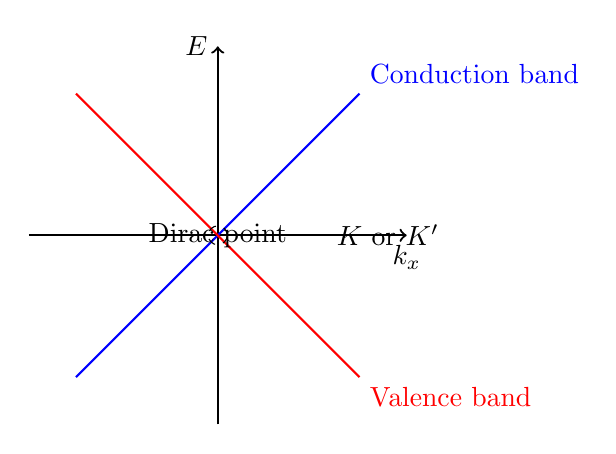
\begin{tikzpicture}[scale=1.2]
\draw[thick,->] (-2,0) -- (2,0) node[below] {$k_x$};
\draw[thick,->] (0,-2) -- (0,2) node[left] {$E$};
\draw[thick,blue] (-1.5,-1.5) -- (1.5,1.5) node[above right] {Conduction band};
\draw[thick,red] (-1.5,1.5) -- (1.5,-1.5) node[below right] {Valence band};
\node at (0,0) {Dirac point};
\node at (1.8,0) {$K$ or $K'$};
\draw[dashed] (0,0) circle (0.1);
\end{tikzpicture}
\caption{Schematic of the Dirac cone in graphene: linear dispersion relation $E = \pm \hbar v_F |k|$ near the Dirac point.}
\label{fig:diraccone}
\end{figure}

Recent advances in encapsulated high-mobility devices have enabled observation of hydrodynamic flow. Key results from Majumdar et al. (Nature Physics, 2025) include a giant violation of the Wiedemann-Franz law and thermal shear viscosity approaching the holographic bound
\[
\frac{\eta_\mathrm{th}}{s_\mathrm{th}} \approx \frac{\hbar}{4\pi k_B}
\]
within a factor of $\sim$4 near room temperature (see Fig.~\ref{fig:viscosity})\cite{majumdar2025}.

\begin{figure}[!htbp]
\centering
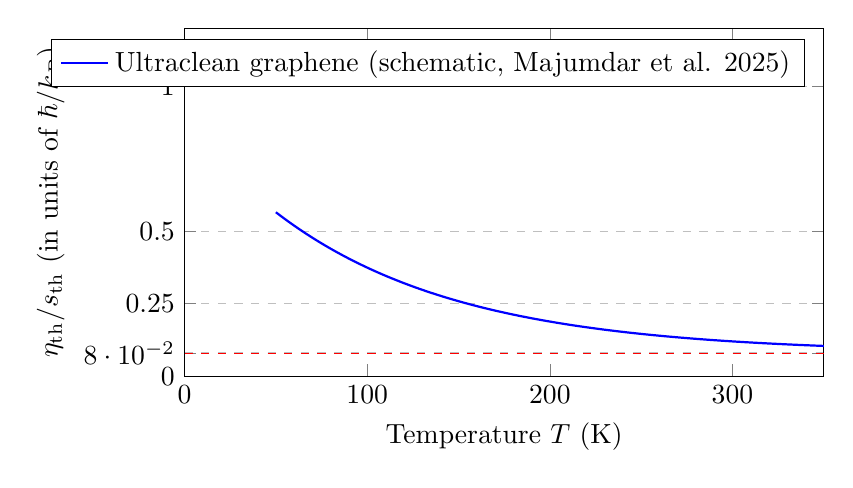
\begin{tikzpicture}
\begin{axis}[
    width=0.8\textwidth,
    height=6cm,
    xlabel={Temperature $T$ (K)},
    ylabel={$\eta_\mathrm{th}/s_\mathrm{th}$ (in units of $\hbar/k_B$)},
    xmin=0, xmax=350,
    ymin=0, ymax=1.2,
    xtick={0,100,200,300},
    ytick={0, 0.08, 0.25, 0.5, 1},
    ymajorgrids=true,
    grid style=dashed,
    legend pos=north east
]
\addplot[
    domain=50:350,
    samples=100,
    thick,
    blue
] {0.08 + 0.8*exp(-x/100)};
\addlegendentry{Ultraclean graphene (schematic, Majumdar et al. 2025)}

\draw[red,dashed] (axis cs:0,0.0796) -- (axis cs:350,0.0796) node[right] {KSS bound $1/(4\pi) \approx 0.08$};

\end{axis}
\end{tikzpicture}
\caption{Schematic plot of thermal viscosity-to-entropy ratio in ultraclean graphene, approaching the Kovtun-Son-Starinets (KSS) bound at higher temperatures.}
\label{fig:viscosity}
\end{figure}

\section{The Kovtun-Son-Starinets (KSS) Bound and Applications in Relativistic Fluid Dynamics}

The Kovtun-Son-Starinets (KSS) bound\cite{kovtun2005} conjectures a universal lower limit on the shear viscosity-to-entropy density ratio for strongly interacting quantum fluids:

\[
\frac{\eta}{s} \geq \frac{\hbar}{4\pi k_B} \approx 0.08 \frac{\hbar}{k_B}
\]

derived from holographic AdS/CFT duality and uncertainty-principle arguments.

Real-world applications include:

\begin{itemize}
\item \textbf{Quark-Gluon Plasma (QGP)}: Created in heavy-ion collisions (RHIC/LHC), the QGP exhibits $\eta/s \approx 0.1 - 0.2$ (in units of $\hbar/k_B$), the closest known system to the bound\cite{heinz2013}.
\item \textbf{Ultraclean Graphene Dirac Fluid}: Near the charge-neutrality point, experiments show $\eta/s \approx 0.3 - 0.8$ near room temperature\cite{majumdar2025, bandurin2016, crossno2016}, approaching the KSS bound within a factor of $\sim$4--10.
\item \textbf{Unitary Fermi Gases}: Cold atoms near unitarity reach $\eta/s \approx 0.4 - 0.5$\cite{cao2011}.
\end{itemize}

These low values highlight universal hydrodynamic behavior in strongly coupled relativistic systems across vastly different energy scales.

\begin{figure}[!htbp]
\centering
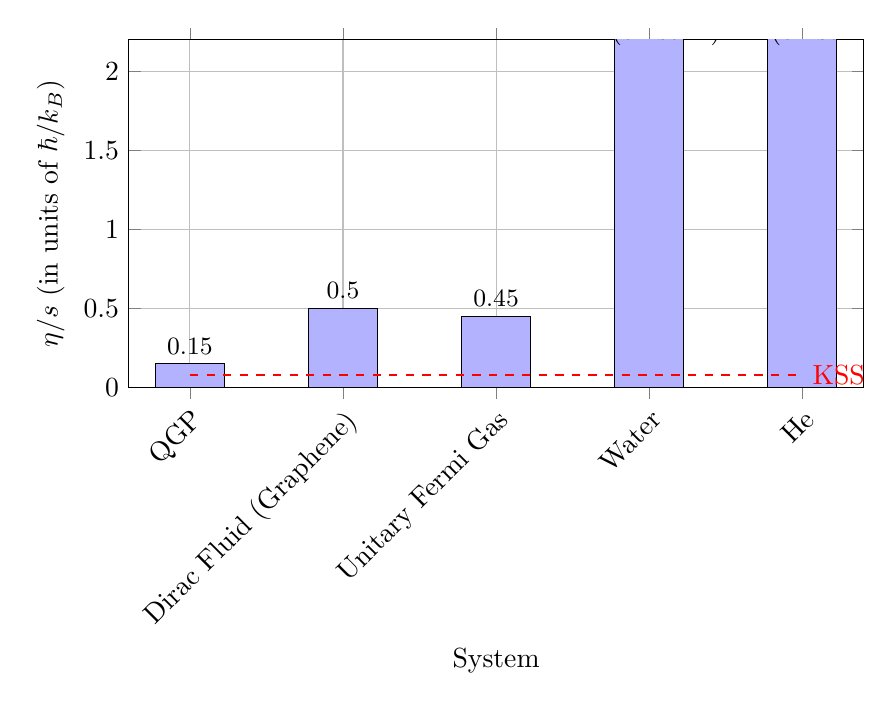
\begin{tikzpicture}
\begin{axis}[
    width=0.9\textwidth,
    height=6cm,  % Ridotta per risparmiare spazio
    xlabel={System},
    ylabel={$\eta / s$ (in units of $\hbar / k_B$)},
    ymin=0, ymax=2.2,
    symbolic x coords={QGP, Dirac Fluid (Graphene), Unitary Fermi Gas, Water, He},
    xtick=data,
    xticklabel style={rotate=45, anchor=north east, inner sep=2pt},
    ybar,
    bar width=25pt,
    grid=major,
    nodes near coords,
    nodes near coords align={vertical},
    every node near coord/.append style={font=\small}
]
\addplot[fill=blue!30] coordinates {
    (QGP,0.15)
    (Dirac Fluid (Graphene),0.5)
    (Unitary Fermi Gas,0.45)
    (Water,10)
    (He,100)
};

\draw[red,dashed,thick] (axis cs:QGP,0.08) -- (axis cs:He,0.08) node[right] {KSS bound $\approx 0.08$};

\node[anchor=south] at (axis cs:Water,2.1) {\small 10 (off-scale)};
\node[anchor=south] at (axis cs:He,2.1) {\small 100 (off-scale)};

\end{axis}
\end{tikzpicture}
\caption{Comparison of $\eta/s$ values across systems (approximate experimental/theoretical averages). The Dirac fluid in graphene approaches the KSS bound, similar to QGP. High values for classical fluids are off-scale.}
\label{fig:ksscomparison}
\end{figure}

\section{Analogies to High-Energy and Gravitational Physics}

The low viscosity and relativistic dispersion mirror properties of the quark-gluon plasma ($\eta/s \approx 1/(4\pi)$) and holographic AdS/CFT duals\cite{kovtun2005}.

\clearpage  % Forza la sezione successiva a iniziare pulita

\section{Speculative Cosmological Connections and Topological Analogies}

This work extends ideas presented in a previous version \cite{soliman2025_zenodo}.
{https://doi.org/10.5281/zenodo.17932055}

Observed local dark matter density lies in the range $\rho_\mathrm{DM} \approx 0.3 - 0.6 \, \mathrm{GeV/cm^3}$\cite{read2014, lim2025}, while galactic magnetic field coherence scales span $\sim$1--10 kpc\cite{planck2016, beck2025}.

Representative values toward the lower end of these ranges (e.g., $\rho_\mathrm{DM} \sim 0.3 \, \mathrm{GeV/cm^3}$, $R_\mathrm{coh} \sim 1$ kpc) align with structural analogies to the ultraclean, near-dissipationless regime of the graphene Dirac fluid\cite{majumdar2025}, where hydrodynamic flow exhibits minimal turbulence and viscosity approaching quantum bounds.

In this ideal limit, topological invariants such as helicity and vortex linking are conserved with high fidelity\cite{moffatt1992, scheeler2014}, evoking speculative parallels to protected braiding in anyonic systems. While no direct emergence of exotic statistics from classical 3D turbulence is established, such analogies highlight universal features of low-dissipation relativistic fluids across scales—from laboratory graphene to cosmological structures.

Future ultra-clean graphene experiments (projected zero-puddle regimes) may further illuminate these connections through enhanced topological protection in electron flow.

\bibliographystyle{unsrt}
\begin{thebibliography}{12}

\bibitem{majumdar2025}
Majumdar, A. et al. Universality in quantum critical flow of charge and heat in ultraclean graphene. \textit{Nat. Phys.} \textbf{21}, 1374--1379 (2025).

\bibitem{novoselov2005}
Novoselov, K. S. et al. Two-dimensional gas of massless Dirac fermions in graphene. \textit{Nature} \textbf{438}, 197 (2005).

\bibitem{kovtun2005}
Kovtun, P., Son, D. T. \& Starinets, A. O. Viscosity in strongly interacting quantum field theories from black hole physics. \textit{Phys. Rev. Lett.} \textbf{94}, 111601 (2005).

\bibitem{read2014}
Read, J. I. The local dark matter density. \textit{J. Phys. G} \textbf{41}, 063101 (2014).

\bibitem{planck2016}
Planck Collaboration. Planck intermediate results. XLII. \textit{A\&A} \textbf{596}, A103 (2016).

\bibitem{heinz2013}
Heinz, U. \& Snellings, R. Collective flow and viscosity in relativistic heavy-ion collisions. Annu. Rev. Nucl. Part. Sci. \textbf{63}, 123 (2013).

\bibitem{bandurin2016}
Bandurin, D. A. et al. Negative local resistance caused by viscous electron backflow in graphene. Science \textbf{351}, 1055 (2016).

\bibitem{crossno2016}
Crossno, J. et al. Observation of the Dirac fluid and the breakdown of the Wiedemann-Franz law in graphene. Science \textbf{351}, 1058 (2016).

\bibitem{cao2011}
Cao, C. et al. Universal quantum viscosity in a unitary Fermi gas. Science \textbf{331}, 58 (2011).

\bibitem{lim2025}
Lim, S. H. et al. Mapping Dark Matter in the Milky Way using Normalizing Flows and Gaia DR3. JCAP \textbf{01}, 021 (2025).

\bibitem{beck2025}
Beck, R. Magnetic fields in the Milky Way and nearby galaxies (review, updated 2025).

\bibitem{moffatt1992}
Moffatt, H. K. \& Ricca, R. L. Helicity and the Călugăreanu invariant. Proc. R. Soc. Lond. A \textbf{439}, 411 (1992).

\bibitem{scheeler2014}
Scheeler, M. W. et al. Complete measurement of helicity and its dynamics in vortex tubes. Science \textbf{344}, 6190 (2014).

\bibitem{soliman2025_zenodo}
Soliman, S. From Ultraclean Graphene to the Cosmological Constant: A Single Measured Scale Unifies Laboratory and Cosmos (TU\_GUT\_SYSY v24). Zenodo \href{https://doi.org/10.5281/zenodo.17932055}{doi:10.5281/zenodo.17932055} (2025).

\end{thebibliography}

\clearpage
\vspace*{2cm}
{\centering
This work is licensed under a Creative Commons Attribution-NonCommercial 4.0 International License (CC BY-NC 4.0).\\
\url{https://creativecommons.org/licenses/by-nc/4.0/}\\
}

\end{document}